\documentclass[11pt]{article}
\usepackage[letterpaper,margin=0.92in]{geometry}
\usepackage[T1]{fontenc}\usepackage{lmodern,amsmath,amssymb,amsthm,booktabs,array,tabularx,longtable,enumitem,microtype,fancyhdr,tikz}
\usetikzlibrary{arrows.meta,positioning}
\usepackage[hidelinks]{hyperref}
\setlength{\parindent}{0pt}\setlength{\parskip}{5pt}\setlist{nosep}
\newtheorem{theorem}{Theorem}[section]\newtheorem{proposition}[theorem]{Proposition}\newtheorem{lemma}[theorem]{Lemma}\newtheorem{corollary}[theorem]{Corollary}
\theoremstyle{definition}\newtheorem{definition}[theorem]{Definition}\newtheorem{example}[theorem]{Example}\newtheorem{conjecture}[theorem]{Conjecture}
\newcommand{\Q}{\mathbb Q}\newcommand{\N}{\mathbb N}\newcommand{\R}{\mathbb R}\newcommand{\E}{\mathbb E}\newcommand{\Prb}{\mathbb P}\newcommand{\Dep}{\operatorname{Dep}}\newcommand{\Ind}{\operatorname{Ind}}\newcommand{\Vfy}{\operatorname{Verify}}\newcommand{\supp}{\operatorname{supp}}\newcommand{\Fix}{\operatorname{Fix}}\newcommand{\eps}{\varepsilon}
\pagestyle{fancy}\fancyhf{}\fancyhead[L]{\small Search Dynamics to SICs}\fancyhead[R]{\small\partlabel}\fancyfoot[C]{\thepage}\setlength{\headheight}{14pt}
\newcommand{\status}[1]{\textbf{Status.} #1}
\newcommand{\partlabel}{Part II / Atlas repeat audit}
\title{From Search Dynamics to Semi-Ideal Computers\\[5pt]\large Part II: The Geometry of Incomplete Proof Knowledge\\\normalsize Certified Envelopes, Active Discovery, and Reliable Feedback}
\author{Picard (AI-assisted research contribution)\\Brian Tenneson, research direction and originating framework}
\date{26 November 2026 (Atlas repeat audit)}
\begin{document}\maketitle
\begin{abstract}
Proof traces reveal legal routes but do not ordinarily reveal the legal routes that were never used. We distinguish observed, possible, and actual theorem-maze geometry by two graph envelopes. On a finite declared edge universe, distances in the possible graph give certified lower bounds and distances in the observed graph give certified upper bounds, provided the outer graph is a certified overapproximation and every retained inner edge has an independently accepted witness. We prove an exact identifiability criterion under an unconstrained completion model, a finite active-query algorithm for closing the distance interval, a worst-case query lower bound, conditional coverage bounds for adaptive trace streams, and robust feedback-control certificates based on interval-valued cost-to-go. The result provides a connection between embedding stability, optimality certification and discovery control without confusing corpus agreement with truth. We distinguish constructive finite results from open transfer questions and report a small exhaustive synthetic enumeration, not an ATP performance benchmark.
\end{abstract}
\textbf{Scope.} This sequel follows the corrected Part I \cite{part1} and the revised Embedding Stability Theorem 7.1 of \emph{Learning Theorem-Space Geometry} \cite{geometry}. Its mathematical statements stand on their own explicit hypotheses. We use no game-theoretic or sovereignty premise, and no claim of unrestricted oraclehood or automatic self-modification.
\clearpage\tableofcontents\clearpage
\section{The missing half of theorem-space learning}
Part I distinguishes the native cost of a proof, the cost of a successful route, and the total computation expended searching. This sequel studies the geometry of the second quantity, relative to a fixed formal presentation. A machine that has observed a ten-step proof knows that a proof of cost at most ten exists. It does not thereby know that every proof costs at least ten. Even a million independently accepted ten-step proofs need not rule out an unobserved two-step proof.

The revised Theorem 7.1 establishes recovery of capped landmark profiles if each corpus eventually covers chosen shortest-path witnesses. The key restriction is coverage: a common estimated geometry may be stable while wrong. Here we ask what an ATP can certify \emph{before} it has such coverage. The answer requires two directions of evidence: witnesses that particular routes are legal, and valid constraints on routes that could still exist. The two directions correspond to upper and lower bounds respectively. Statistical agreement may guide acquisition of either kind of evidence; it does not establish the missing inequality.
\section{A finite proof-geometry information state}
Fix a finite state set $V$ of complete proof states, a frozen goal set $Z\subseteq V$, and a finite universe $U$ of candidate directed edges, with known exact nonnegative rational cost $w(e)$ for each candidate. Parallel edges are allowed with distinct labels. The unknown actual legal graph $G=(V,E)$ satisfies $E\subseteq U$. The representation contract must establish this inclusion; a guessed candidate list is not a certified outer universe. Costs and state identity are shared across all observations. Each edge label must identify a legal transition between the declared complete states, with its cost. The representation contract must also ensure that local witnesses concatenate along a walk with matching states, including all proof contexts and dependencies; the empty walk is legal at a goal. For interpreting a route as a theorem proof, a walk from the declared entrance to a goal must decode to an independently accepted certificate at the stated route cost, and every in-scope admissible proof route must be represented if optimality over those routes is claimed. The graph results below are valid as graph statements without a logical decoding, but their ATP interpretation requires these additional contracts. A formal verifier accepts certificates of legality; a separate justified decision procedure or certificate checker may establish illegality of a candidate in the fixed scope. Rejection of one proposed proof witness is not in general proof that an edge is illegal.
\begin{definition}[Certified edge information]
At time $n$, let $L_n$ be the set of edges certified legal and $N_n$ the set certified illegal. The unresolved set is $Q_n=U\setminus(L_n\cup N_n)$. Soundness means $L_n\subseteq E\subseteq U\setminus N_n$. Both evidence sets grow by verified deposits, with disjointness preserved. Write $G_n^-=(V,L_n)$, $G_n^+=(V,U\setminus N_n)$.
\end{definition}
Here the superscripts refer to edge inclusion, not numerical distance. The information state can be stored as a monotone typed ledger in the SIC sense of Part I. Its projection need not determine the next acquisition action; the operational controller may also need queues, a learning model, and a budget. A graph envelope may be produced by a sound abstract interpretation instead of candidate-by-candidate testing, provided its cost-relaxation contract proves the lower inequality. The edge-universe model is used below for the stronger identifiability and query results.
\begin{center}
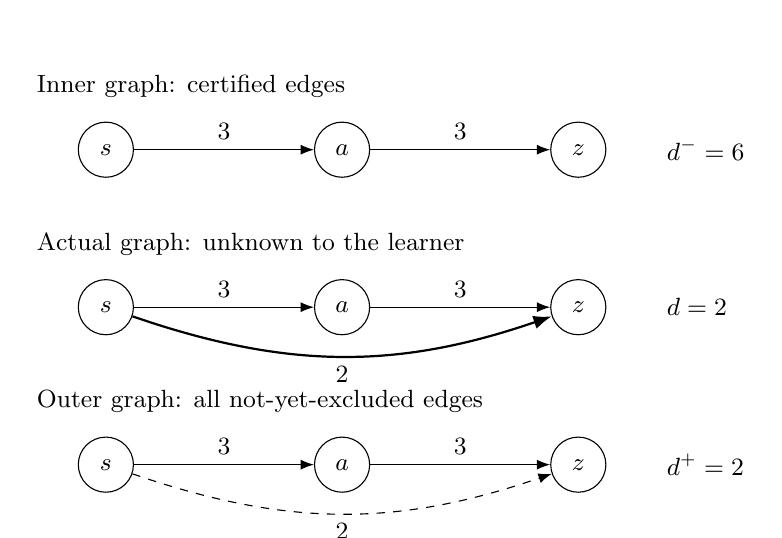
\begin{tikzpicture}[>=Latex,every node/.style={font=\small},x=1cm,y=1cm]
\foreach \y/\lab in {4/{Inner graph: certified edges},2/{Actual graph: unknown to the learner},0/{Outer graph: all not-yet-excluded edges}}{
\node[anchor=west] at (0,\y+.8){\lab};
\node[draw,circle,minimum size=7mm] (s\y) at (1,\y){$s$};\node[draw,circle,minimum size=7mm] (a\y) at (4,\y){$a$};\node[draw,circle,minimum size=7mm] (z\y) at (7,\y){$z$};
\draw[->] (s\y)--node[above]{3}(a\y);\draw[->] (a\y)--node[above]{3}(z\y);
}
\draw[->,thick] (s2) to[bend right=19] node[below]{2} (z2);
\draw[->,dashed] (s0) to[bend right=19] node[below]{2} (z0);
\node[anchor=west] at (8,4){$d^-=6$};\node[anchor=west] at (8,2){$d=2$};\node[anchor=west] at (8,0){$d^+=2$};
\end{tikzpicture}
\end{center}
The dashed edge is possible, not established by the data. The actual graph in this illustration contains it, but a different actual graph without the shortcut is also compatible with the same evidence. The learner knows only $2\le d(s,Z)\le6$ until the shortcut is resolved.
\section{The two-envelope theorem}
For each vertex $v$ put
\[\ell_n(v)=d_{G_n^+}(v,Z),\qquad u_n(v)=d_{G_n^-}(v,Z).\]
Distances take values in $[0,\infty]$, with $\infty$ for unreachable exits. If a real-valued representation is wanted, fix a cap $R>0$ and apply $r\mapsto\min(r,R)$ to all distances. A cap is not a claim of reachability.
\begin{theorem}[Certified distance envelopes]\label{thm:env}
For every $v$ and every $n$,
\[\ell_n(v)\le d_G(v,Z)\le u_n(v).\]
The lower bound is nondecreasing and the upper bound is nonincreasing as sound evidence grows. Equality $\ell_n(v)=u_n(v)<\infty$ certifies the exact route optimum and an inner-graph path attaining it. Equality at $\infty$ certifies unreachability in the declared finite scope. The inequalities and monotonicity also hold after capping. Equality of the capped endpoints at a common value strictly below $R$ certifies an exact finite optimum and an inner path attaining it. Equality at $R$ certifies only $d_G(v,Z)\ge R$; it certifies neither reachability nor unreachability.
\end{theorem}
\begin{proof} Graph inclusion reverses shortest-path distance: enlarging a graph adds admissible paths without changing the weights of old ones. Apply this to $G_n^-\subseteq G\subseteq G_n^+$ and to consecutive inner and outer graphs. Finite graphs with nonnegative edge costs attain any finite optimum after cycle deletion. The cap is order preserving.\end{proof}
Define the capped uncertainty width $W_n(v)=\min(R,u_n(v))-\min(R,\ell_n(v))$. This is nonnegative and nonincreasing. For a fixed probability distribution $\nu$ on the fixed finite state set and a fixed cap $R$, $I_n=\sum_v\nu(v)W_n(v)$ is one mathematically explicit measure of \emph{geometric uncertainty}. It is not logical ignorance in general, nor a measure of every unknown theorem. It depends on the scope, target, cost, cap, and workload. Zero width for one goal says nothing about other goals. It may be zero even if many legal edges remain unknown.
\section{When is the geometry identifiable?}
\begin{definition}[Completion model]
Given $L,N$, an unconstrained admissible completion is any $E'$ with $L\subseteq E'\subseteq U\setminus N$. Under a constrained model $\mathcal C$, require additional verified relations among candidates (e.g. a symmetry or inference rule linking edge statuses). A completion model represents uncertainty about the graph, not a collection of alternative truths in one fixed fully specified calculus.
\end{definition}
\begin{theorem}[Sharp identifiability criterion]\label{thm:id}
In the unconstrained completion model, the possible values of $d_{E'}(v,Z)$ have attained minimum $\ell(v)$ and attained maximum $u(v)$, including the extended value $\infty$. Hence the distance is identifiable from the evidence exactly when $\ell(v)=u(v)$. The same equivalence holds for capped profiles and for simultaneous identification of a finite list of pairs (coordinate by coordinate).
\end{theorem}
\begin{proof} Every completion lies between the two envelope graphs, so Theorem~\ref{thm:env} bounds its distances. The extreme graphs with edge sets $U\setminus N$ and $L$ are themselves completions. They attain the two extremes. Thus if these differ, two compatible graphs disagree, while equality forces every completion to agree. Apply the monotone cap and repeat for each pair.\end{proof}
With constraints, the two extremes need not be feasible completions. The envelopes remain valid but may be conservative. Exact identifiability then means equality of minimum and maximum over the nonempty finite feasible completion set. Enumerating that set may be exponential. Proof systems normally impose dependencies; the unconstrained theorem is a precise information-theoretic abstraction, not an assertion that any subset of formal inferences is a possible calculus.
\begin{corollary}[No uniformly accurate point estimate without evidence]
In the unconstrained completion model of Theorem~\ref{thm:id}, if the two capped endpoints differ by $W>0$, any deterministic real-valued estimate based solely on this information state has maximum absolute error at least $W/2$ for the capped distance over the compatible graphs. The midpoint attains that worst-case bound for this single coordinate.
\end{corollary}
\begin{proof} The two extreme compatible values differ by $W$, so the triangle inequality forces at least one error to be at least $W/2$. Every compatible value lies in the interval and is at most $W/2$ from its midpoint.\end{proof}
This explains a failure mode of independently trained embeddings: two models can fit the same stable inner geometry and still agree at the wrong value. A free latent coordinate need not be unique even when all distances are known. A canonical landmark-distance profile avoids rotations and arbitrary latent alignments, but does not magically recover unobserved routes.
\section{An active discovery algorithm}
Suppose in the finite declared universe there is a total, sound procedure that resolves a queried edge as legal or illegal with an accepted witness. This is an explicit strong assumption. A normal proof checker that only accepts submitted derivations does not automatically implement it. Unresolved queries in a practical ATP must be logged as unresolved, not counted as illegal. With total resolution we can certify a target distance without resolving all edges.
\begin{theorem}[Optimistic-path resolution]\label{thm:active}
Fix $s,Z$. While $\ell(s)<u(s)$, choose a minimum-cost simple $s$--$Z$ path in the outer graph and resolve one unresolved edge on that path. Update the evidence and repeat. This process closes the distance interval in at most $|Q_0|$ resolutions. At closure it certifies either an optimal feasible route or unreachability in the declared scope.
\end{theorem}
\begin{proof} If $\ell<u$ then $\ell<\infty$, so a finite optimal outer path exists. If every edge of that path belonged to $L$, it would be an inner path of cost $\ell$ and would imply $u\le\ell$, a contradiction. Hence a queried unresolved edge exists. A sound resolution strictly decreases $|Q|$. If $Q$ is empty the two graphs coincide. Each step preserves the envelopes, and Theorem~\ref{thm:env} certifies the final answer.\end{proof}
The controller may choose the most promising unresolved edge on the optimistic path using learned predictions, anticipated verification cost, or expected influence on other goals. It cannot turn an unverified prediction into an exclusion. A practical extension with partial resolution may schedule other queries and fall back on fair proof search; the finite resolution bound does not transfer unless unresolved edges on required witnesses can eventually be settled.
\begin{theorem}[A worst-case query obstruction]
In the independent-edge query model, there exist graphs with $m$ unresolved edges for which any always-correct distance-certifying algorithm requires $m$ edge resolutions in the worst case, even with a known feasible incumbent.
\end{theorem}
\begin{proof} Give $s$ and $z$ a known legal edge of cost 2, and $m$ distinguishable unresolved parallel edges of cost 1. The actual graph with none of the cheap edges has optimum 2. Until every cheap edge is ruled out, the compatible graph containing an unresolved cheap edge has optimum 1. An always-correct algorithm cannot certify 2 on the all-negative instance before all $m$ queries. The argument also holds for a randomized algorithm required to be correct for every realized query history.\end{proof}
The finite upper bound in Theorem~\ref{thm:active} is therefore sharp in the worst case for this oracle model. All stopping tests in this algorithm use uncapped distances; equality at the cap is not an exact-optimality certificate. It is not a polynomial-time theorem in the size of an implicit logical input: the universe may be huge and edge resolution itself may be expensive. The value of targeted acquisition is that it can stop early when remaining uncertainty has no influence on the desired distance.
\section{Certificates for lower bounds and optimality}
There is a concise way to independently check finite shortest-path lower bounds without trusting the search implementation.
\begin{theorem}[Potential certificate]\label{thm:potential}
Let $h:V\to\Q_{\ge0}$ satisfy $h(z)=0$ for every $z\in Z$ and
\[h(v)\le w(v,v')+h(v')\]
for every edge of a certified outer graph. Then $h(v)\le d_G(v,Z)$ for each $v$. If a verified actual path from $s$ to $Z$ costs $h(s)$, it is optimal in the declared scope.
\end{theorem}
\begin{proof} Sum the inequalities along any actual path (which lies in the outer graph). The potential terms telescope to $h(s)-h(z)=h(s)$, giving $h(s)\le w(P)$. Infimize. A verified path of equal cost gives the opposite inequality.\end{proof}
A finite-cap variant always has finite values: for a positive rational cap $R$, $h(v)=\min(R,d_{G^+}(v,Z))$ satisfies the inequalities, including at unreachable states. The proof follows from the distance triangle inequality and nonnegative weights, with the cap handled by cases. Thus the exact rational capped outer distance gives a concrete potential certificate. For an unreachability certificate use a reachable set containing $s$, disjoint from $Z$, and closed under all outer edges. A small proof object may be a symbolic proof of the edge inequalities or closed-set property; it must cover every outer edge, not merely those previously generated by the search; verifying an explicit huge edge universe need not be cheap. This is the dual counterpart to the path witness. An observed shortest path by itself supplies no such certificate.
\begin{proposition}[Safe frontier intervals]
For any reached path-label $(v,g)$ and incumbent $B$, if $g+\ell(v)\ge B$ then this label cannot strictly improve $B$. If a path to $v$ of cost $g$ and a finite inner route of cost $u(v)$ are verified and concatenation is legal in the complete state encoding, $g+u(v)$ is a feasible incumbent candidate.
\end{proposition}
\begin{proof} The lower assertion uses Theorem~\ref{thm:env} and nonnegative additive route costs. The upper assertion concatenates the legal walks.\end{proof}
This turns geometric learning into a certificate-producing search strategy. An ML model can propose a potential, but it becomes a lower bound only when the checker has verified its inequalities on the complete outer representation. An upper bound must carry a route, not merely a regression estimate. Exact graph algorithms and learned frontier ordering can coexist without confusing the two types of evidence.
\section{From embedding stability to adaptive coverage}
Fix the actual graph, a finite ordered landmark set $A\subseteq V$, and cap $R>0$. All observations in this section contain only actual legal edges and the accumulated inner graph is persistent. Let $\Phi(v)=(\min(R,d_G(v,a)))_{a\in A}$. Define coordinatewise inner and outer profiles from the two graphs, taking each landmark as its own target. Choose one shortest witness for each pair $(v,a)$ with $d_G(v,a)<R$, and let $W$ be their finite union of edges, $m=|W|$. In the earlier article, independent traces with positive coverage yielded eventual equality of inner profiles. The following strengthens the observation model without assuming independence between traces.
\begin{theorem}[Adaptive witness coverage]\label{thm:coverage}
Let the $n$th observation be an arbitrary adaptive verified trace, with history $\mathcal F_{n-1}$. Suppose for each $e\in W$ not yet observed,
\[\Prb(e\text{ appears at step }n\mid\mathcal F_{n-1})\ge p_n\quad\text{a.s.},\]
where $p_n\in[0,1]$ is deterministic. Let $\Phi_n^{\rm in}$ be the inner profile after $n$ observations. Then
\[\Prb(\Phi_n^{\rm in}\ne\Phi)\le\min\left(1,m\prod_{j=1}^n(1-p_j)\right).\]
If $\sum_n p_n=\infty$, almost surely all inner profiles equal the actual profile eventually and thereafter. For $k$ corpora with possibly dependent streams, a union bound gives $m\sum_{c=1}^k\prod_{j=1}^n(1-p_{c,j})$ (capped at 1), with their respective conditional coverage lower bounds.
\end{theorem}
\begin{proof} For a fixed edge let $M_n$ be its missing event through step $n$. Then $\Prb(M_n)\le(1-p_n)\Prb(M_{n-1})$ by conditioning and the fact that a missing edge must have been missing previously. Iterate, then take a union bound. Once every selected witness edge appears, each subcap distance has its exact witness in the inner graph, and at-cap coordinates already equal the cap. The product tends to zero if the sum diverges, so each edge is eventually observed with probability one. Finiteness of $W$ makes the last observation time finite almost surely. No cross-corpus independence is used.\end{proof}
This extends the prior finite-witness theorem to adaptive trace distributions. It does not assert the conditional lower bound for real ATPs. For example a scheduler that samples one search wing infinitely often need not give every edge a positive chance if that wing never traverses some shortest path. If $p_n$ is summable, infinite trace count alone does not force full coverage. For instance, independent trials with one required edge appearing with probability $2^{-n-1}$ at round $n\ge1$ satisfy the conditional lower bound but have strictly positive probability of missing that edge forever, since the infinite product of the complementary probabilities is positive. A simple sufficient design in finite scope is a background acquisition policy with a known positive probability of each selected witness edge on each allocated round; the exploration probabilities must have divergent total mass. If the guarantee only concerns observed paths, the actual inner profile may converge before the learner can certify that it has converged. Outer evidence supplies that missing certificate.
\begin{corollary}[Certified profile stability without a sampling theorem]
For any two learners with sound envelopes on the same graph, shared landmarks and shared cap, use the finite capped interval endpoints in each coordinate. If their coordinate widths are at most $\delta_1,\delta_2$, respectively, then their midpoint profiles differ coordinatewise by at most $(\delta_1+\delta_2)/2$. Each midpoint is within half its own width of the actual coordinate.\end{corollary}
\begin{proof} The actual coordinate belongs to both intervals. Use the midpoint error bounds and the triangle inequality.\end{proof}
Unlike raw inter-corpus agreement, this comparison comes with an error witness. The unknown geometry is used only in the proof of the bound, not as an input to computing the midpoint. Learned representations can fit these intervals rather than invent a unique target distance from incomplete data. Learned errors measured on held-out traces are still empirical unless bounded uniformly by an appropriate proof.
\section{Reliable feedback under interval uncertainty}
Part I repairs the stochastic Bellman objective by requiring positive nonterminal costs and finite expected cost from each state (or a separately proved properness contract). Here we use that finite-state model: a known transition kernel $K$, nonempty finite action sets at nonterminal states, absorbing $Z$ with zero terminal cost, finite costs $0<c_0\le c(x,a)\le c_1<\infty$ outside $Z$, and finite optimal expected cost $V^*$ at every state. All history-dependent randomized policies are admissible, and the pre-transition filtration includes the chosen action, as in Part I. Deterministic graph distances are a special case with actions selecting legal edges, provided the positive-cost and finite-value hypotheses hold. In a stochastic system the graph of possible transitions alone does not determine expected cost; the following interval hypotheses concern actual $V^*$, not shortest support-graph distances. They must be established by a separate value certificate, exact model computation or robust relaxation.

Let $\underline V\le V^*\le\overline V$ be certified finite bounds. Define for every action
\[L_a(x)=c(x,a)+\E[\underline V(X')\mid x,a],\quad U_a(x)=c(x,a)+\E[\overline V(X')\mid x,a].\]
Write $Q^*(x,a)=c(x,a)+\E V^*(X')$. Every action interval encloses $Q^*(x,a)$.
\begin{theorem}[Certified action and regret]\label{thm:action}
If $U_a(x)\le L_b(x)$ for every $b\ne a$, then $a$ is optimal (uniquely if strict). For any selected action $a$, a valid bound on regret $Q^*(x,a)-V^*(x)$ is
\[r(x,a)=U_a(x)-\min_b L_b(x).\]
If every executed action at every nonterminal reachable state has $r(x,a)\le\rho<c_0$, then $\E_x\tau\le V^*(x)/(c_0-\rho)$ and the policy reaches $Z$ almost surely. Moreover its expected cost exceeds $V^*(x)$ by at most $\rho\E_x\tau$.
\end{theorem}
\begin{proof} The interval ordering implies $Q^*(x,a)\le Q^*(x,b)$ for each competitor. The regret bound follows from $Q^*(x,a)\le U_a$ and $V^*(x)=\min_b Q^*(x,b)\ge\min_b L_b$. From the Bellman equation the conditional expected decrease in $V^*$ under the chosen action equals $c(x,a)$ minus the true regret, at least $c_0-\rho$. The stopped drift theorem of Part I applies. For the cost gap, telescope $Q^*(X_t,a_t)-V^*(X_t)=c_t+\E[V^*(X_{t+1})\mid\mathcal F_t]-V^*(X_t)$ until $n\wedge\tau$. Finite state space gives bounded $V^*$, and the hitting-time bound and bounded costs give finite expected accumulated cost. Pass to the limit: the terminal potential vanishes in expectation and total expected regret is at most $\rho\E\tau$.\end{proof}
The robust bound requires coverage of the executed states and actions. A certificate at one initial decision does not establish the entire trajectory. A narrow value interval at the current state alone is also insufficient; the relevant interval widths lie at successor states. For exact kernels, choosing the smallest upper action value is a conservative policy, but without a uniform regret margin there is no unconditional hitting-time guarantee from that rule alone.
\begin{proposition}[A checkable stochastic lower/upper pair]\label{prop:stoch}
In the same finite positive-cost model, let $h\ge0$ be finite with $h=0$ on $Z$ and $h(x)\le c(x,a)+\E[h(X')\mid x,a]$ for every nonterminal action. Let $g\ge0$ be finite with $g=0$ on $Z$, and suppose a fixed selector $\pi$ satisfies $g(x)\ge c(x,\pi(x))+\E[g(X')\mid x,\pi(x)]$ for every nonterminal state. Then $h\le V^*\le V^\pi\le g$ and $\pi$ is proper.
\end{proposition}
\begin{proof} Telescope the inequality for $h$ along an optimal proper policy (whose existence follows from Part I), up to $n\wedge\tau$. Bounded $h$ and almost-sure stopping remove the terminal expectation; the expected cost tends to $V^*$. For $g$, the expected decrease is at least $c_0$, so the stopped drift theorem gives $\E\tau\le g(x)/c_0$. Telescoping the supersolution inequality bounds expected cost by $g(x)$; optimality of $V^*$ gives the middle comparison.\end{proof}
These are ordinary Bellman inequalities with an explicit stopping proof. They suggest a way of producing stochastic interval certificates from approximate Abel coordinates: propose $h$ and a selector with $g$, check inequalities exactly for rational finite kernels, and use the resulting intervals only if the checks succeed. In the deterministic case these reduce to lower potentials and feasible route costs. They are not automatic certificates for neural networks or continuous unbounded state spaces.
\section{A reproducible finite experiment}\label{sec:experiment}
We now test the logic of the acquisition procedure on a deliberately tiny finite universe. Use vertices $s,a,b,z$, known edges $s\to a$ and $a\to z$ of cost 3 each, and six candidate edges in the fixed order:
\begin{center}\begin{tabular}{clc}\toprule ID&Candidate&Cost\\\midrule
0&$s\to z$&2\\1&$s\to b$&1\\2&$b\to z$&1\\3&$a\to b$&1\\4&$b\to a$&1\\5&$s\to a$ (parallel macro)&2\\\bottomrule\end{tabular}\end{center}
Each of the $2^6=64$ candidate-status masks is treated once as the actual graph; all have an incumbent route of cost 6. This is exhaustive enumeration of a synthetic family, not independent draws from a theorem population. Compare two controllers with the same unit-cost exact membership query and stop test: (A) query the lowest-ID unresolved edge on a lexicographically tie-broken optimistic shortest path; (B) query unresolved edges in fixed ID order regardless of the current path. Both stop when $\ell=u$. The oracle is simulated by the mask. An independent shortest-path computation on the full actual graph checks the claimed distance in every case. Record all 64 results, including query count and target optimum. No neural training, natural theorem corpus or wall-clock improvement is measured.

\begin{table}[ht]\centering
\begin{tabular}{lrr}\toprule Outcome & Active optimistic path & Fixed order\\\midrule
Exact certificates &64/64&64/64\\
Total queries &164&196\\
Mean queries per mask &2.5625&3.0625\\
Minimum / maximum queries &1 / 5&1 / 6\\
\bottomrule\end{tabular}
\caption{Executed exhaustive finite experiment, all 64 masks.}\end{table}
The active policy used fewer queries in 24 masks, tied in 40, and used more in none. Its counts at 1, 3, 4, 5 queries were respectively 32, 8, 12, 12. Fixed order used 1, 3, 5, 6 queries in respectively 32, 8, 4, 20 masks. Actual optima were 2 in 40 masks, 4 in 2, 5 in 14, and 6 in 8. The numerical distance sandwich was checked at every iteration, and every final equality agreed with a separate Bellman--Ford relaxation implementation on the actual graph. The Atlas v2 re-execution reproduced all 64 CSV rows exactly and all aggregate counts. The full CSV and standard-library script accompany this paper.

The main experimental point is not superiority of a particular tie-break rule. It is that the exact stopping certificate permits a reproducible test of which questions mattered. Query order can reduce the number of resolved edges, but the cost of generating the outer universe and checking the negative facts is not modeled here. The complete enumeration is small enough to repeat without statistical assumptions. The companion Python script is a standard-library implementation, not a formal proof assistant verification of the theorems.
\section{The next research program}
Part I's reported H2 experiment has a binary endpoint tied for all five intervention families. Rather than treat geometric progress as a replacement for settlement, a new prospective experiment should ask whether certificate-bearing interventions reduce uncertainty width or close an optimality gap before binary success. A proposed design has four stages.
\begin{enumerate}[leftmargin=*]
\item Start with finite symbolic mazes whose full legality relation is independently computable. Compare observation-only upper bounds, certified outer potentials, active path resolution, and a learned query ordering. Charge all oracle, search, and verification costs separately.
\item Move to finite bounded fragments of formal proof systems in which a complete candidate universe can be justified (for example explicit grammar, depth, and bounded substitutions). Do not call a truncated grammar complete for the ambient calculus. Log legal, illegal and unresolved evidence with scope hashes.
\item Use independent proof corpora with shared canonical states or a proved translation. Compare landmark profiles and their certified intervals on held-out targets. Estimate coverage empirically, but do not assume Theorem~\ref{thm:coverage}'s hypothesis solely because the observed learning curve saturates.
\item On sealed stochastic or deterministic control tasks, learn candidate potentials and action orderings only from earlier audited targets. Check interval or Bellman certificates before deployment. Compare certified progress, actual discovery rates, query effort and total resource costs, with fair exact-search fallback and prospectively declared budgets. Preserve failed runs.
\end{enumerate}
\begin{conjecture}[Sparse decisive evidence]
There exist nontrivial families of formal proof mazes with efficiently representable outer relaxations for which active acquisition of a small number of certified constraints closes a target distance interval at substantially lower total cost than exhaustive graph construction.
\end{conjecture}
\begin{conjecture}[Transferable uncertainty guidance]
For some independently generated theorem families sharing a certified representation, a frozen predictor of width reduction per unit of acquisition cost improves total certified settlement or optimality-certification effort relative to matched nonlearned acquisition policies.
\end{conjecture}
Both claims are open in this manuscript. The first depends on compact certificates and effective negative information; the second requires prospective cross-family evidence. One must not infer either from the 64-mask model or the earlier 20-target compass diagnostics. An alternative possibility is that useful outer relaxations are too weak or too costly for important natural families. In that case the obstruction should be recorded, and proof search should fall back on verifier-safe exact or heuristic ordering rather than treating a statistical model as an authority.
\section*{Atlas v2 audit addendum}
The re-audit separated capped and uncapped optimality statements, specified the unconstrained completion model for the minimax bound, restricted midpoint comparisons to finite capped coordinates, and required a rational cap for rational potential certificates. The stochastic section now explicitly imports the finite-state policy and filtration contracts of the audited Part I. The adaptive sampling theorem is stated on a fixed actual graph with persistent sound observations; no cross-corpus independence is needed. The 64-mask experiment was rerun from the supplied code and its complete CSV matched the supplied results. A second proof pass found no unresolved defect under the revised finite hypotheses. The natural-theorem efficiency and transfer conjectures remain open; this review is not a machine proof or independent peer review.
\section*{Atlas repeat-audit addendum (26 November 2026)}
This pass starts from the previously audited v2. The edge-evidence contract now explicitly requires composable state witnesses and cost-preserving decoding and coverage for the interpretation of graph optima as proof optima. The stochastic control section states the finite upper cost bound used in its proof, the summable-coverage limitation has an explicit counterexample, and the experimental wording describes the precise numerical invariant checked by the code. The supplied finite experiment was rerun and compared against its original CSV. The proofs and their dependencies on Part I were reread under the repaired contracts. No claim of natural-ATP acceleration or machine-checked proof is added.
\section{Conclusion: discovery includes learning what cannot be shorter}
The central mathematical object in this sequel is not a point estimate of distance but a pair of certified bounds. A verified proof answers an existence question. A lower-bound witness answers a different question: how much shorter could a proof still be? The two together can certify an optimum, and the interval between them gives a precisely scoped quantity of remaining uncertainty. The active acquisition theorem demonstrates how one may target this uncertainty without requiring exhaustive recovery of every edge. The adaptive coverage theorem shows how stable landmark geometry can emerge from nonindependent search traces under declared coverage; the countermodel theorem shows why it cannot be assumed to emerge. Finally the interval feedback theorem gives a conditional path from geometry certification to reliable control.

The natural next frontier is a formal proof calculus with a cheap, justified outer relaxation, in which a machine can learn which facts are worth certifying rather than merely which known proofs are worth imitating. This remains a research objective. Its value is that failure is itself mathematically interpretable: an unknown shortcut, a loose outer relaxation, a missing certificate language, or an action gap too small to control safely.
\section*{Provenance and AI-integrity statement}
This article is an AI-assisted mathematical research sequel in the Picard conversational role. The source program is Brian Tenneson's original Part I (v0.4a) and the corrected edition, together with the earlier embedding-stability article. The envelope, active-query, adaptive-coverage and interval-control statements are proved here under their declared assumptions; several use established graph, interval and stochastic shortest-path principles. No assertion of priority or literature-exhaustive novelty is made. The synthetic enumeration was executed as described; neither natural-mathematics acceleration nor unrestricted inference is claimed. The prose proofs have received Picard self-review and a subsequent AI-assisted Atlas audit, not independent peer review or machine checking. No change to an underlying AI model or verifier is asserted.
\small\begin{thebibliography}{99}
\bibitem{part1} B. Tenneson, with Picard, \emph{From Search Dynamics to Semi-Ideal Computers, Part I: Theorem Mazes, Certified Settlement, and Feedback Control}, corrected research edition v0.5, Atlas repeat audit, 26 Nov. 2026.
\bibitem{geometry} B. Tenneson, with Picard, \emph{Learning Theorem-Space Geometry}, Picard v2, 25 Nov. 2026, especially Theorem 7.1.
\bibitem{dijkstra} E. W. Dijkstra, A note on two problems in connexion with graphs, \emph{Numer. Math.} 1 (1959), 269--271. \href{https://doi.org/10.1007/BF01386390}{doi:10.1007/BF01386390}.
\bibitem{astar} P. E. Hart, N. J. Nilsson, B. Raphael, A formal basis for the heuristic determination of minimum cost paths, \emph{IEEE Trans. Syst. Sci. Cybern.} 4(2) (1968), 100--107. \href{https://doi.org/10.1109/TSSC.1968.300136}{doi:10.1109/TSSC.1968.300136}.
\bibitem{ssp} D. P. Bertsekas, J. N. Tsitsiklis, An analysis of stochastic shortest path problems, \emph{Math. Oper. Res.} 16(3) (1991), 580--595. \href{https://doi.org/10.1287/moor.16.3.580}{doi:10.1287/moor.16.3.580}.
\bibitem{leandojo} K. Yang et al., LeanDojo: Theorem proving with retrieval-augmented language models, NeurIPS 2023, \url{https://arxiv.org/abs/2306.15626}. A related proof-environment and data extraction resource, not evidence for the conjectures here.
\end{thebibliography}
\end{document}
